\documentclass[runningheads,a4paper]{llncs}
%\documentclass[letter,11pt]{article}
%geometry -> one inch marge.
\usepackage{./sty/mystyle}

\usepackage{url}
\urldef{\mailsa}\path|mateusz.lacki@biol.uw.edu.pl|
\urldef{\mailsb}\path|aniag@mimuw.edu.pl|

\newcommand{\keywords}[1]{\par\addvspace\baselineskip
\noindent\keywordname\enspace\ignorespaces#1}

\begin{document}
\mainmatter  

\title{IsoDittwald\\Law of Localised Mass Spec Fine Structure}

\titlerunning{IsoDittwald}

\author{Mateusz \L\k{a}cki\thanks{Special thanks to Santa Claus.}
\and Anna Gambin}

\authorrunning{IsoDittwald}


% the affiliations are given next; don't give your e-mail address
% unless you accept that it will be published
\institute{
  Faculty of Mathematics, Informatics and Mechanics\\ University of Warsaw, Banacha 2, 02-097 Warszawa, Poland\\
  \mailsa\\
  \mailsb\\
  \url{http://bioputer.mimuw.edu.pl}
}

% NB: a more complex sample for affiliations and the mapping to the
% corresponding authors can be found in the file "llncs.dem"
% (search for the string "\mainmatter" where a contribution starts).
% "llncs.dem" accompanies the document class "llncs.cls".

\toctitle{IsoDittwald}
\tocauthor{Mateusz \L\k{a}cki}
\maketitle

\begin{abstract}
  Approximative distributions theory is used to obtain more tractable formulas describing the localised fine structure of isotopic peaks.  
  We present a new method for calculating localised fine structure isotopic peaks based on the above-mentioned approximations. 
\emph{abstract} environment.
\keywords{Isotopic Fine Structure, Poisson Approximation, Little Sexy Fox}
\end{abstract}

% \listoftodos

%!TEX root = ../DeGaulle.tex
\section{Introduction}

There are many reasons why mass spectrometry analysis is hard. It is hard in that there are potentially many many sources of interferences that can distort the information about the actual composition of a sample. The study of the nature of these interferences is needed to achieve the goal of making out of mass spectrometers yet more reliable an identification tool. 

Part of the noise in the mass to charge domain is innately related to the elements themeselves and stems from the existence of isotopes. It is because of them that a given analyte is represented as a series of peaks, a spectrum, rather that only one peak. The theoretical underpinnings of how to mathematically model the impact of isotopes are already well established, see \cite{Valkenborg2012Isotopic}. The main idea behind the model is to abstract from the exact positionings of the extra neutrons on a particular chemical compound and thus concentrate only on their relative amounts among all atoms of a given element. Assuming that the isotopic configurations are independent and follow the element dependent distribution, one arrives to the conclusion  that the correct law describing occurence of different isotopes in a chemical compound is the product of multinomial distributions. 

There is one huge problem with that law: together with the growth of molecule one observes an exponential growth in the number of possibile isotope configurations, which precludes their direct enumeration. To solve this problem, different semplifications were proposed, amounting to different ways of binning configurations together explicitly \cite{Claesen2012Efficient}, by hiding them under the guise of Fourier Transform \cite{Rockwood1995Relationship}, or by \dots 

\todo[inline]{Add Olson and others but Olson above all.}

Here we propose to approach the problem of fine structure so that it overcomes the shortcomings of the aggregate model, as used in \cite{Claesen2012Efficient}. That particular model bins together configurations having the same number of extra neutrons distributed on different atoms. For instance, if one considers water molecule \ce{H_2 O}, the model would glue together configuration with one extra neutron only on the first hydrogen togeter with that having it on the second together with that on oxygen atom. We devise an algorithm to deaggregate these probability clusters. We call the peaks obtained via that algorithm a {\it localised fine structure}. 


What motivates the solution to this problem is a search for better molecule fingerprints. The development of new mass spectrometers capable of distinguishing differences in masses of neutrons is proceeding at a vigorous pace. Soon, scientists will face the need of more detailed models than those abstracting from mass defects. It is also common for chemists to search for presence of specific substance in the sample. Usually this is done by looking at some highly specific range in the mass domain of the gathered spectra. Our model provides deeper insight to what might happen while focussing on that particular bit of collected data: conditioning on configurations with the same number of extra neutrons translates directly into focussing in a specific region of the mass-to-charge domain.


The algorithm assumes that one can easily find a peak not far from the most probable one and that the distribution is close to what one would call unimodal\footnote{We provide a precise definition of unimodality for discrete probability distributions in Section \dots} and that the most of distributions probability lies in a rather small neighbourhood of the mode. Both the guess about the starting point and the way the neighbourhood gets explored depend on the Poisson approximation to the distribution under study. To our best knowledge this type of approximation have not yet been used for algorithmic purposes. It has been used however in the context of proteomic and peptide research: in \cite{Breen2000AutomaticPeak} it is being used for high throughput protein identification; its use was revalidated in \cite{Valkenborg2007UsingPoisson} in case of peptides.


We also observe that the use of Poisson approximation gives a theoretical explanation for the equatransneutronic binning used in \cite{Olson2009Calculations} and actually helps deaggregating results obtained using that approach as well.



% For instance, by neglecting the fact that the mass of additional neutron with respect to the lightest isotope can discriminate between elements, one arrives at a probability distribution that is computationally tractable in different ways: either algebraically \cite{Claesen2012Efficient}, by use of Fourier Transform \cite{Rockwood1995Relationship}, dynamic programming , Li2008HierarchicalAlgorithm  


% The main idea is to treat a chemical compound, such as \molecule, as a set of 

% The problem is that usually a more detailed approach 

% There is usually much of indeterminacy in the 
% Part of the problem lies in the nature of chemical sound that prohibits us from getting to know the exact composition of an analyte under study. One must acknowledge also the fact, that part of indeterminacy in the obtained results stems from the existence of isotopes of different elements. Mass 

% A result of a mass spectrometry experiment is usually a complicated spectrum 

% The concept of isotopic structure is crucial for the proper interpretation of mass spectrometry spectra. 

% The fact that the result of a mass spec analysis is usually an entire spectrum in the mass to charge domain rather than an individual peak can to some extent be attributed to the existance of the isotopic structure. 

% Part of the indeterminacy in the mass to charge domain can be attributed to the existence of isotopes.

% In this article we are asking ourselves a question of how to 

% The interpretation of a mass spectrometry analysis is rarely trivial, the number of possible sources of  interferences being a very large one. Even a perfectly carried out experiment usually  

 % of a given analyte rarely does appear in mass spec spectra in form of a single peak and a lot of the indeterminacy in weight can be attributed to the existence of isotopes.  


	% Cite all others.



% One of the first uses of Poisson approximation in the context of isotopic structure calculations is to be found in \cite{Breen2000AutomaticPeak}, where it is being used for high throughput protein identification. The use of approximation was validated in \cite{Valkenborg2007UsingPoisson} in case of peptides. Authors of this article also raise the important topic of approximations validity, from a purely applied viewpoint. 





% All interesting citations \cite{Claesen2012Efficient} and \cite{Valkenborg2012Isotopic} and \cite{Olson2009Calculations} and \cite{Ipsen2014Efficient} and \cite{Valkenborg2008ModelBased} and \cite{Valkenborg2007UsingPoisson} and \cite{Rockwood1995Relationship} and \cite{Breen2000AutomaticPeak}.
%!TEX root = ../DeGaulle.tex
\section{Approximations}

By an isotopic configuration we understand information about the number of different isotopes in the sample. For the purpose of simplicity, we focus here on chemical compounds composed of carbon, hydrogen, nitrogen, oxygen, and sulfur; still, the results of this section generalize to any compounds whatsoever. Thus, we concentrate on compounds like \molecule, where the low case letters describe the numbers of atoms of particular element type. Among such compounds one can already find peptides and proteins. An isotopic configuration could be represented by an extended empirical formula, 
\begin{equation}\label{long chemical formula}
	\text{\moleculeIsotopic}.
\end{equation}

In the above representation, small letters with indices represent counts of different atoms with indices displaying the number of additional neutrons an isotope has with respect to the lighest possible isotopic variant. 

Rather than \eqref{long chemical formula}, we shall be using an equivalent probabilistic notation, treating upper case letters, like \ce{^{12}C}, as random variables and considering small case letters, $\cem{c_0}$, to be their realisations. An expression like $A = \{ \ce{^{13}C} = \cem{c_1},\, \ce{^{2}H} = \cem{h_1} \}$ is shorthand for saying: let us focus on all configurations \eqref{long chemical formula} that have \ce{c_1} heavy carbons and \ce{h_1} deuters in total.


Following \cite{Kienitz1961MassSpectrometry}, one assumes that the law of vector
\begin{equation}\label{long chemical vector}
	\left( \cem{^{12}C},\, \cem{^{13}C},\, \cem{^{1}H},\, \cem{^{2}H},\, \cem{^{14}N},\, \cem{^{15}N},\, \cem{^{16}O},\, \cem{^{17}O},\, \cem{^{18}O},\, \cem{^{32}S},\, \cem{^{33}S},\, \cem{^{34}S},\, \cem{^{36}S} \right),	
\end{equation}
given \molecule, is a product of independent multinomial distributions,
{\small\begin{equation}\label{product of multinomials}
	\MM = \mathrm{Multi} \Big( \prob(\cem{^{12}C}), \prob(\cem{^{13}C}); c \Big)
	\otimes \dots \otimes 
	\mathrm{Multi} \Big( \prob(\cem{^{32}S}), \prob(\cem{^{33}S}), \prob(\cem{^{34}S}), \prob(\cem{^{36}S}); s \Big),	
\end{equation}}
where the probabilities of observing particular isotopes, $\prob(\cem{^{12}C})$, \dots, $\prob(\cem{^{36}S})$, are established in independent experiments\footnote{Consult Table \ref{basic info on isotopes table} for details.}. For instance, the probability of a given carbons configuration $(\cem{c_0}, \cem{c_1})$ equals
% \begin{equation*}
% 	\mathrm{Multi} \left( \prob(\cem{^{12}C}), \prob(\cem{^{13}C}); c \right)
% 		\Big( (\cem{c_0}, \cem{c_1}) \Big) = 
% 	\begin{pmatrix}
% 		\cem{c} \cr \cem{c_0}, \cem{c_1}  
% 	\end{pmatrix} \prob(\cem{^{12}C})^\cem{c_0} \prob(\cem{^{13}C})^\cem{c_1}
% \end{equation*}
$$
	\mathrm{Multi} \left( \prob(\cem{^{12}C}), \prob(\cem{^{13}C}); c \right)
		\Big( (\cem{c_0}, \cem{c_1}) \Big) = 
	\begin{pmatrix}
		\cem{c} \cr \cem{c_0}, \cem{c_1}  
	\end{pmatrix} \prob(\cem{^{12}C})^\cem{c_0} \prob(\cem{^{13}C})^\cem{c_1}
$$
and it should be multiplied by similar expression for hydrogen, nitrogen, oxygen and sulfur to obtain probability for expression like \eqref{long chemical formula}.


Observe, that given \molecule, part of the information in \eqref{long chemical vector} is redundant and can be shortened by neglecting counts of the lightest isotope variants, leaving us with 
\begin{equation}\label{short chemical vector}
 	\left( \cem{^{13}C},\, \cem{^{2}H},\, \cem{^{15}N},\, \cem{^{17}O},\, \cem{^{18}O},\, \cem{^{33}S},\, \cem{^{34}S},\, \cem{^{36}S} \right).	
\end{equation}
Missing therms can be retrieved from relationships $\cem{^{12}C} + \cem{^{13}C} = \cem{c}$, $\cem{^{1}H} + \cem{^{2}H} = \cem{h}$, and so on, that occur with probability one.

\begin{mydef}\label{localised fine structure definition}
	We call the set of configurations  
	{\small
		\begin{equation}\label{LFS_K}
			LFS_K	=
			\left\{ 
				\cem{^{13}C} + \cem{^{2}H} +  \cem{^{15}N} +  \cem{^{17}O} +  \cem{2 $\times$^{18}O} +  \cem{^{33}S} +  \cem{2 $\times$^{34}S} + \cem{4 $\times$^{36}S} = K	
			\right\}
		\end{equation}
	}
	a \emph{localised fine structure with $K$ extra neutrons}.  	
\end{mydef}

The reason for numbers 2 and 4 appearing above is that \ce{^{18}O} and \ce{^{34}S} have two additional neutrons, and \ce{^{36}S} -- four; confront Table \ref{basic info on isotopes table}.

The problem of finding the cardinal number of $LFS_K$ is also known as the money exchange problem. In general, enumeration of all elements of $LFS_K$ corresponds to finding all integer solutions $(x_1, \dots, x_k)$ to a {\it Linear Diophantine Equation}  
\begin{equation}\label{Linear Diophantine Equation}
	d_1 x_1 + \dots + d_k x_k = K,
\end{equation}
where $(d_1, \dots, d_k)$ are integer coefficients. According to \cite{Agnarsson2002OnTheSylvesterDenumerants}, if the greatest common divisor of $(d_1, \dots, d_k)$ is equal to one, then the number of solutions to \eqref{Linear Diophantine Equation} is approximately $\frac{K^{k-1}}{(k-1)! d_1 \dots d_k}$. Carbon has only one addtional isotope, so $\exists_i d_i = 1$ in \eqref{Linear Diophantine Equation}. The above estimate encompases therefore all of organic chemistry. 

The problem is big, being polynomial in $K$. Nevertheless, configurations in $LFS_K$ are naturally prioritized by probability \eqref{product of multinomials}. Rather than enumerating them all, one can be satisfied with only the most probable ones. 

%  is simply a subset of all possible configurations \eqref{long chemical formula} with additional constraint 
% \begin{equation}\label{Simple Diophantine Equation}
% 	\cem{c_1} + \cem{h_1} + \cem{n_1} + \cem{o_1} + 2 \cem{o_2} + \cem{s_1} + 2 \cem{s_2} + 4 \cem{s_4} = K.
% \end{equation}

\begin{Problem}\label{Problem of finding LFS_K configurations.}
	For a given $K$, find a small set $B \subset LFS_K$ of configurations s.t. 
	\begin{equation}\label{problem equation}
		\MK (B) := \frac{ \MM(B) }{ \MM( LFS_K ) } \approx 1\,,	
	\end{equation} 
	where $\MK$ is the product of multinomial laws \eqref{product of multinomials} conditional on the set of configurations in $LFS_K$ and is refered to as \emph{The Law of Localised Fine Structure}.
\end{Problem}


In statistical terms, we are interested in approximating some critical set of large probability, as measured by the {\it Law of Localised Fine Structure}. 


Why should one study law described by \eqref{problem equation} in the first place? Simply because the masses of different configurations in $LFS_K$ concentrate around the compound's monoisotopic mass shifted to the right by $K$ Daltons\footnote{For underlying physical principles consult \cite{Hughey2001KendrickMassDefect}.}. For medium sized compounds, $LFS_K$'s for different $K$ should in principle form disjoint clusters in the mass to charge domain, as argued in manuscript \cite{Dittwald2014OnTheFineIsotopicDistribution}; for bigger compounds some interference would be expected, but in that case one would simply study three or more consecutive sets of configurations, e.g. $LFS_{K-1}$, $LFS_K$, and $LFS_{K+1}$. All in all, by studying $LFS_K$ we get a guarantee to explore thoroughly a precised place in the mass to charge domain. More reasons behind this idea are exposed in the \textbf{Conclusions and Discussion} section. 


To solve Problem \ref{Problem of finding LFS_K configurations.} we approximate measure $\MK$ by a more analytically tractable measure $\QK$ defined on the $LFS_K$. We then devise an algorithm to find a possibly small set of configurations $B^* \subset LFS_K$, s.t. $\QK (B^*) \approx 1$. Since $\QK \approx \MK$, so $\MK (B^*) \approx 1$ and $B^*$ solves Problem \ref{Problem of finding LFS_K configurations.}, possibly suboptimally.


A natural way to define proper $\QK$ is to first approximate $\MM$ by some $\QQ$ and then pose $\QK (\circ) := \frac{\QQ (\circ \cap LFS_K) }{\QQ(LFS_K)}$, i.e. condition $\QQ$ on the occurence of configurations from $LFS_K$. To prove it works, we have to first mention, that by approximation we understand convergence in distribution, as described in \cite{Kallenberg2002FoundationsOfModernProbability}. Then, we make use of the following lemma: 

\begin{lemma}\label{conditional convergence lemma}
	Let $\mu^{[n]}, \mu$ be discrete measures. If $\mu^{[n]}$ converges in distribution to $\mu$, $\mu^{[n]} \rightharpoonup  \mu$, and an event $A$ has nonzero probability under any of that measures, $\underset{n}{\forall} \mu^{[n]}(A)\,,\, \mu(A) > 0$, then measures conditioned by $A$, $\mu^{[n]}_A (\circ) := \frac{\mu^{[n]} ( \circ \cap A)}{\mu^{[n]}(A)}$ converge in distribution to $\mu_A (\circ) := \frac{ \mu( \circ \cap A) }{ \mu(A) }$; or $\mu^{[n]}_A \rightharpoonup \mu_A$ for short.
\end{lemma}  
The proof is exposed in the \textbf{Appendix}.  


Let us now unveil the usefulness of Lemma \ref{conditional convergence lemma}. There is an entire family of measures mentioned in it, $\mu^{[n]}$. We assume, that one of them is simply our initial meausure: there exists $n^*$ s.t. $\MM = \mu^{[n^*]}$. Also, we assume the approximation of $\mu^{[n^*]}$ by measure $\mu$ is already o good one. Our choice for $\mu$ is to be the product of independent Poisson measures, which is stimulated by the following, well known lemma\footnote{ The proof is common knowledge and we omit it.}.


\begin{lemma}\label{weak convergence of multinomial to Poissons lemma}
	If all\,\,$\lim_{n\to \infty} n p_{k,n}= \lambda_k$ exist for $k \in \{1,\dots, w\}$, then 
	
	\begin{equation}\label{weak convergence of multionial to Poissons equation}
		\mathrm{Multi}\left( p_0^{[n]}, p_1^{[n]}, \dots, p_w^{[n]}; n \right) 
			\rightharpoonup 
		\mathrm{Poiss}( \lambda_1) \otimes \dots \otimes \mathrm{Poiss}( \lambda_w ),	
	\end{equation}
	where $\mathrm{Poiss}$ stands for the Poisson distribution, $\mathrm{Poiss}(\lambda)(k) 	= \frac{\lambda^k}{k!}e^{-\lambda}$.
	
\end{lemma}


In Lemma \ref{weak convergence of multinomial to Poissons lemma} one assumes that the number of trials $n$ goes to infinity. In our model this corresponds to an infinite enlargement of the compound. The existence of limits assumes that this enlargement is done so that on such an idealized compound only the lightest isotopes would appear infinitely often. Moreover, since the support of any Poisson distibution is equal to the set of all integer numbers, the state space of configurations gets significantly enlarged and contains configurations that are nonphysical for any real chemical compound. For instance, positive probabilities would be prescribed to configurations with numbers of isotopes greater then the number of possible places for them on any finite compound\footnote{There is no mathematical incongruence here, however, since the approximation assumes that the limiting compound is of infinite size. For mathematical correctness we also note, that we can transfer virtually any initial measure $\MM$ on the enlarged state space, i.e. where the approximation is defined, simply by assuming, that $\MM$ measure on any nonphysical configuration equals zero.}. Observe also, that the probabilities $p_k^{[n]}$ are pending towards zero: for good approximation one would expect therefore the probabilities of observing heavier isotopes, e.g. quantities like $\prob(\cem{^{13}C}), \prob(\cem{^{2}H}), \dots, \prob(\cem{^{36}S})$, to be relatively small. Confront Table \ref{basic info on isotopes table} to check, that this is really the case.


Observe, that Lemma \ref{weak convergence of multinomial to Poissons lemma} defines a proper limit for just one multinomial distribution, whereas $\MM$ is a product thereof. The problem is other than what to do with products: one can approximate independently each multinomial. However, the quality of such approximation depends on all the counts of different elements in a molecule. For instance, in case of \molecule\,the better the approximation\footnote{The {\it goodness} of approximation is expressed in the total variance distance; see \cite{Roos1999OnTheRateOfMultivariatePoissonConvergence}.} the bigger the smallest among numbers $(\cem{c}, \cem{h}, \cem{n}, \cem{o}, \cem{s})$. Due to the polymer structure, one would expect some more information could be reveiled on that matter for proteins and peptides. Indeed, empirical research by Senko et al. \cite{Senko1995Determination} established the concept of avergine, i.e. an averaged protein: any protein composed of $m$ amino acids should have its mass approximately equal to the mass of the idealised compound 
\begin{equation*}
	\cem{C}_{\lfloor m \times 4.9384\rfloor} 
	\cem{H}_{\lfloor m \times 7.7583\rfloor} 
	\cem{O}_{\lfloor m \times 1.4773\rfloor} 	
	\cem{N}_{\lfloor m \times 1.3577\rfloor} 
	\cem{S}_{\lfloor m \times 0.0417\rfloor}.
\end{equation*}

The weakest link in the approximation might result from small numbers of sulfur. This is an acknowledged problem in empirical studies, as exposed in \cite{Valkenborg2007UsingPoisson}. The longer the polymers however, the smaller the differences should be. 


The final questions is: what values should be used as $\lambda$'s in Lemma \ref{weak convergence of multinomial to Poissons lemma}? We {\it calibrate} those values by equating them to the averages of the multinomial distributions from \eqref{product of multinomials}\footnote{Such {\it calibration} is common practice in statistics.}: in case of carbon we set $\lambda_\cem{^{13}C} \approx \cem{c} \times \prob( \cem{^{13}C} )$.  In contrast to our method, $\lambda$'s in \cite{Breen2000AutomaticPeak,Valkenborg2007UsingPoisson} are chosen to be the minimisers in a free parameter optimisation scheme with $\chi^2$ penalty\footnote{Note however, that these two solutions should not differ too much for larger compounds, for it is known that both the Poisson and Multinomial distributions are concentrated near their means, see \cite{Bobkov1998OnModifiedLogarithmicSobolev}.}. 


At days end, the probability assigned to event
\begin{equation*}
 	\left\{ \cem{^{13}C} = \cem{c_1},\, \cem{^{2}H} = \cem{h_1},\, \cem{^{15}N} = \cem{n_1},\, \cem{^{17}O} = \cem{o_1},\, \cem{^{18}O} = \cem{o_2},\, \cem{^{33}S} = \cem{s_1},\, \cem{^{34}S} = \cem{s_2},\, \cem{^{36}S}= \cem{s_4} \right\}	
\end{equation*} 
is given by
\begin{equation}\label{QK Nominator}
	\poiss{\text{c}}{13}{1}
	\poiss{\text{h}}{2}{1}
	\poiss{\text{n}}{15}{1}
	\poiss{\text{o}}{17}{1}
	\poiss{\text{s}}{33}{1}
		e^{ - \mu}
	\poiss{\text{o}}{18}{2}	
	\poiss{\text{s}}{34}{2}
		e^{ - \eta }		
	\poiss{\text{s}}{36}{1}
		e^{ - \gamma },
\end{equation}
where 
\begin{align*}\label{intensities summed equation}
	\mu 	&=	\lambda_\cem{^{13}C} + \lambda_\cem{^{2}H} + \lambda_\cem{^{15}N} + \lambda_\cem{^{17}O} +\lambda_\cem{^{33}S}  	\\
	\eta 	&= 	\lambda_\cem{^{18}O} + \lambda_\cem{^{34}S}\\ 
	\gamma	&= 	\lambda_\cem{^{36}S}.
\end{align*}

The usefulness of approximation by a product of independent Poisson lies in two important properties, as summarised in the following lemmas.

\begin{lemma}\label{sum of independent Poissons lemma}
	Suppose we have a collection of $m$ independent Poisson-distributed random variables, $X_i \sim \mathrm{Poiss}(\kappa_i)$. Then $X_1 + \dots + X_m \sim \mathrm{Poiss}(\kappa_1 + \dots + \kappa_m)$. 
\end{lemma}  

\begin{lemma}\label{Poisson conditional on sum of Poissons}
	Suppose we have a collection of $m$ independent Poisson-distributed random variables, $X_i \sim \mathrm{Poiss}(\kappa_i)$. Then $X_1, \dots, X_m$ given that $X_1 + \dots + X_m = K$ is multinomially distributed,

$$ 
	\Big(X_1, \dots, X_m | X_1 + \dots + X_m = K \Big) 
	\sim 
	\mathrm{Multi}\Big( \frac{\kappa_1}{\sigma}, \dots, \frac{\kappa_m}{\sigma}; K \Big), 
$$
	where $\sigma = \sum_{i = 1}^m \kappa_i$.	
\end{lemma}
Both lemmas are proved in \cite{Kingman1993PoissonProcesses}. Lemma \ref{sum of independent Poissons lemma} shows how to semplify calculations for a Diophantine equations with all parameters set to one, $a_i \equiv 1$. Lemma \ref{Poisson conditional on sum of Poissons} describes the law resulting from conditioning independent Poisson variables by such an expression. 

Suppose that we concentrated on molecules composed entirely of elements that can have only one additional neutron, e.g. \smallMolecule. By Lemma \ref{Poisson conditional on sum of Poissons} we get:

\begin{result}\label{Multinomial Result}
 	For \smallMolecule, let $\tilde{\mu} := \lambda_\cem{^{13}C} + \lambda_\cem{^{2}H} + \lambda_\cem{^{15}N}$. Then
 	$$\QK = \mathrm{Multi}\left(
 		\frac{\lambda_\cem{^{13}C}}{\tilde{\mu}}, 
 		\frac{\lambda_\cem{^{2}H}}{\tilde{\mu}}, 
 		\frac{\lambda_\cem{^{15}N}}{\tilde{\mu}}; K \right).$$
\end{result}

\begin{proof}
	The corresponding Diophantine equation is $\cem{^{13}C} + \cem{^2H} + \cem{^{15}N}$.
\end{proof}

It is valuable to see, how Lemma \ref{Poisson conditional on sum of Poissons} generalizes while conditioning on a more complex Diophantie equation. Observe, that \eqref{LFS_K} can be rewritten as 
\begin{equation*}
	LFS_K = \Big\{ \underbrace{\cem{^{13}C} + \cem{^2H} + \cem{^{15}N} + \cem{^{17}O} + \cem{^{33}S}}_{ G_1 } + \,2 \times \underbrace{( \cem{^{18}O} + \cem{^{34}S} )}_{ G_2 } + \,4 \times \underbrace{\cem{^{36}S}}_{ G_4 } = K \Big\},	
\end{equation*}
so that in light of Lemma \ref{sum of independent Poissons lemma}, $\QQ(A)$ can be calculated in an easier way: 
$$\QQ( LFS_K ) = \sum_{k_1 + 2 k_2 + 4 k_4 = K} \prob( G_1 = k_1, G_2 = k_2, G_4 = k_4 ),$$
where $G_1 \sim \mathrm{Poiss}( \mu )$, $G_2 \sim \mathrm{Poiss}( \eta )$, and $G_4 \sim \mathrm{Poiss}( \gamma )$ are mutually independent. There is a strict link between $G_i$ and the concept of {\it equatransneutronic groups} described in \cite{Olson2009Calculations}: it is equal to the total number of atoms bearing exactly $i$ additional neutrons.  

To calculate $\QK$ it remains to divide \eqref{QK Nominator} by $\QQ( LFS_K )$. Observe however that a more significant expression is to be obtained, if additionally we multiply both the nominator and the denominator of that expression by $\frac{\mu^{k_1}}{k_1 !} \frac{\eta^{k_2}}{k_2 !} \frac{\gamma^{k_4}}{k_4 !}$:

% Note also, that 
% \begin{align*}
% 	x 	& = \cem{c_1} + \cem{h_1} + \cem{n_1} + \cem{o_1} + \cem{s_1}, \\	  	
% 	y 	& = \cem{o_2} + \cem{s_2}, 	\\
% 	z 	& = \cem{s_4}.
% \end{align*}
% In \cite{Olson2009Calculations} they are encoded by $k_1, k_2$, and $k_4$; also, $d_{G_i} = i$. Then it is true that

\begin{result}\label{Fine structure law}
	The approximative \emph{fine structure law} with $K$ additional neutrons for \molecule\, is equal to 
	{\small
		\begin{equation*}
			\mathrm{Multi} \left(
				\frac{ \lambda_\cem{^{13}C} }{ \mu }, 
				\frac{ \lambda_\cem{^{2} H} }{ \mu }, 
				\frac{ \lambda_\cem{^{15}N} }{ \mu },
				\frac{ \lambda_\cem{^{17}O} }{ \mu }, 
				\frac{ \lambda_\cem{^{33}S} }{ \mu }; 
				k_1
			\right ) \otimes
			\mathrm{Multi} \left(
				\frac{ \lambda_\cem{^{18}O} }{ \eta },
				\frac{ \lambda_\cem{^{34}S} }{ \eta }; 
				k_2	
			\right) \otimes 
			\mathbb{L}( k_1, k_2, k_4 ),
		\end{equation*}
	}
	where 
	\begin{equation}\label{simple lucky law}
		\mathbb{L}( k_1, k_2, k_4 ) = 
		\frac{ \frac{ \mu^{k_1} }{ k_1! } \frac{ \eta^{k_2}}{ k_2! } \frac{ \gamma^{k_4} }{ k_4! } }{ 
			\underset{ k_1' + 2 k_2' + 4 k_4' = K}{\sum} 
				\frac{ \mu^{k_1'} }{ k_1'! } 
				\frac{ \eta^{k_2'}}{ k_2'! } 
				\frac{ \gamma^{k_4'}}{ k_4'! }
		}.
	\end{equation}
\end{result}

Otherwise stated, the approximative distribution is a mixture of independent multinomial distributions weighted by the $\mathbb{L}$ distribution, which, for lack of name, we shall call the {\it lucky law}. Under the Poisson approximation, the {\it lucky law} is the resulting law on the {\it equatransneutronic configurations}.

If the compound contains elements with their {\it additional neutron acceptances} in set $I = \{ 1, 2, 4\}$, formula \eqref{simple lucky law} generalizes to 
\begin{equation*}
	\mathbb{L}( \bm{k} ) = 
	\frac{ 
		\prod_{i \in I} \frac{ \mu_i^{k_i} }{ {k_i}! } 
	}{ 
		\underset{ \{ \bm{k}^* :  \sum_{i \in I} i k_i^*  = K \} }{\sum} 	
		\prod_{i \in I} \frac{ \mu_i^{k_i^*} }{ {k_i^*}! }	
	},
\end{equation*}
where $\bm{k}$ is an ordered tuple indexed by $I$. Nature poses a natural limit on the complexity of the {\it lucky law}, as at most  $\# I \leq 10$\todo{Ascertain that asking Frederik.}.
%!TEX root = ../DeGaulle.tex
\section{Algorithms}

Results \ref{Fine structure law} and \ref{Equatransneutronic Masses result} open up a new way to do calculations: using the approximation one reduces the complexity of Problem \ref{Problem of finding LFS_K configurations.} to that of studying $\mathbb{L}$. The {\it lucky law} is usually defined on a less dimensional space than $\MK$ and that significantly reduces the  computational effort. In proteomics, the state space of $\mathbb{L}$ can be thought to be two-dimensional, making it possible to establish the mass and probability of every {\it equatransneutronic grouping} in a {\it double for loop}. This approach is described as Algorithm \ref{DeFiner code}, code-named \textsc{DeFiner}. In general, exploration of $\mathbb{L}$ could be achieved by a tailored MCMC algorithm.   

\begin{algorithm}\caption{\textsc{DeFiner}}\label{DeFiner code}
\begin{algorithmic}\label{DeFiner Parallely}
	\State	\textbf{Input:}\,\,\,\,\, \molecule, $K$
	\State 	\textbf{Output:} A triplet of arrays with configurations, their probability, and mass.
	\State 	Establish $\lambda_\cem{^{13}C}, \lambda_\cem{^{2} H}, \lambda_\cem{^{15}N}, \lambda_\cem{^{17}O}, \lambda_\cem{^{33}S}, \mu, \gamma $, and all mass differences $\Delta M$.
	\State 	Find   $S = \{ (k_1, k_2, k_4) : k_1 + 2 k_2 + 4 k_4 = K \}$.
	\FORALL{ $\bm{k} \in S$}
		\State 	$\mathrm{Lucky}(\bm{k}) := \mathbb{L}\Big( \{ \bm{k} \} \Big)$
		\State 	$M(\bm{k}) :=$ mass of configuration $\bm{k}$ obtained using Eq. \eqref{Equatransneutronic masses eq} 
	\ENDFORALL
	\State 	Return $\{ S, \mathrm{Lucky}, M\}$.
\end{algorithmic}	
\end{algorithm}

\textsc{DeFiner} can be used as a subroutine for \textsc{DeFinest}: an algorithm that provides the exact multinomial peaks. \textsc{DeFinest} works as follows. 

First, having obtained the {\it lucky} configurations, we order them in descending $\mathbb{L}$-probability and select the critical $L\%$-set $S_L$ to trim out the asymptotically negligible configurations. To show it is so, let us introduce some extra notation
\begin{equation}
	\bm{g}_1 := (\cem{c_1}, \cem{h_1}, \cem{n_1}, \cem{o_1}, \cem{s_1} ), \quad
	\bm{g}_2 := (\cem{o_2}, \cem{s_2}), \quad
	g_4 := \cem{s_4}, \quad 
	\bm{g} := ( \bm{g}_1, \bm{g}_2, g_4)
\end{equation}
We think of $\bm{g}_1$ and $\bm{g}_2$ as of configurations of the multinomial laws described in Result \ref{Fine structure law}. Observe that entries of $\bm{g}_i$ sum to $k_i$. By Result \ref{Fine structure law}, note that $\QK \big( S_L \big) \leq \QK \big( S \big) = \mathbb{L}\big( \{ \bm{k} \} \big)$, where $\bm{k} := (k_1, k_2, k_4)$, the probability of a peak in a given {\it equatransneutronic grouping} being smaller than the probability of all the peaks gathered in it. Therefore, asymptotically all the $\bm{g}$ configurations in $S_L$ have a small $\QK$-probability, and we can decide whether to neglect them using only the information contained in $\mathbb{L}\big( \{ \bm{k} \} \big)$.

Subsequently, for each configuration $\bm{k}$ in $S_L$, one independently identifies critical $M\%$-set $\mathfrak{M}$ and critical $B\%$-set $\mathfrak{B}$ of the two underlying multinomial distributions. This can be achieved in many ways, see \textbf{Appendix} for our approach. With these sets at hand we calculate their exterior product and obtain a set of valid configurations from $LFS_K$. We then find their true $\MK$-probability and their mass $M$ using Eq. \eqref{Equatransneutronic masses eq}. We make use of \textsc{BRAIN} \cite{Dittwald2013BRAIN} software to get $\MM(LFS_K)$ needed to calculate $\MK$. Finally, we merge all obtained solutions.

Say that the algorithm resulted in set $A$ of configurations. One can measure \textsc{DeFinest}'s performance simply by calculating the overall $\textsc{Coverage} := \MK(A)$; the higher it is, the better we are in solving Problem \ref{Problem of finding LFS_K configurations.}.

A prototype of \textsc{DeFinest} has been implemented in \textbf{R}. Its pseudo code is described as Algorithm \ref{DeFinest code}. Observe also, that the {\it for loop} can be carried out in parallel. Fig. \ref{figure: Coverage} shows how well the prototype manages in solving Problem \ref{Problem of finding LFS_K configurations.}. 




\begin{algorithm}\caption{\textsc{DeFinest}}\label{DeFinest code}
\begin{algorithmic}
	\State	\textbf{Input:} \molecule, $K, L, M, B$
	\State 	\textbf{Output:} array of masses and probabilities, \textsc{Coverage}.
	\State 	Run \textsc{DeFiner} and obtain $\{ S, \mathrm{Lucky}, M\}$.
	\State 	$S_L$:= top $L\%$ of configurations from $S$ ordered by their {\it lucky probabilities}, $\mathbb{L}(\{ \bm{k} \})$.
	

	\FORALL{ $\bm{k} \in S_L$}
		\State $\mathfrak{M}$ := Critical $M\%$ set of $\mathrm{Multi} \left(
				\frac{ \lambda_\cem{^{13}C} }{ \mu }, 
				\frac{ \lambda_\cem{^{2} H} }{ \mu }, 
				\frac{ \lambda_\cem{^{15}N} }{ \mu },
				\frac{ \lambda_\cem{^{17}O} }{ \mu }, 
				\frac{ \lambda_\cem{^{33}S} }{ \mu }; 
				k_1
			\right )$

		\State $\mathfrak{B}$ \,:= Critical $B\%$ set of 
		$\mathrm{Multi} \left(
			\frac{ \lambda_\cem{^{18}O} }{ \eta },
			\frac{ \lambda_\cem{^{34}S} }{ \eta }; 
			k_2	
		\right)$		

		\State $\mathfrak{R}_{\bm{k}}$ := $ 
			\Bigg\{ 
				\Big( 
					\MK( \bm{g} ), 
					M( \bm{g} )
				\Big) : \bm{g} = ( \bm{g}_1, \bm{g}_2, g_4 ) \in \mathfrak{M} \otimes \mathfrak{B} \otimes \{ k_4 \}  
			\Bigg\}$, cf. Eq. \eqref{Equatransneutronic masses eq} 
	\ENDFORALL

	\State 	Find {\sc Coverage}.
	\State 	Return $\big\{ \bigcup _{\bm{k}} \mathfrak{R}_{\bm{k}}, \textsc{Coverage} \big\}$.
\end{algorithmic}	
\end{algorithm}
%!TEX root = ../DeGaulle.tex
\section{Conclusions}

	In the present paper an original approach to doing calculations on different levels of isotopic fine structure aggregation hierarchy was proposed. To our best knowledge, it is the first use of Poisson approximation for algorithmic purposes,   resulting already in two elegant algorithms, \textsc{DeFine} and \textsc{DeFiner}, for efficient exploration of the state space of possible isotopic configurations.  

	\textsc{DeFine} is a minimalistic, yet extremely efficient way of calculating approximate probabilities of {\it equatransneutronic} clusters. \textsc{DeFiner} presents a simple but certainly suboptimal way of handing Problem \ref{Problem of finding LFS_K configurations.}; however, more efficient algorithms can easily come into being by more careful considerations on how to explore the approximative distribution $\QK$. 

	Figure \ref{figure: hierarchy} presents a detailed view of the hierarchical approach we take. The left pane contains the  aggregated isotopic distribution of \testAvergine, an $100$-avergine, obtained with the {\sc BRAIN} algorithm \cite{Dittwald2013BRAIN}. The lower panel zooms into the region of the highest aggregated peak. This peak is then desaggregated into {\it equatransneutronic} groupings. Finally, one notices many small black peaks corresponding to the finest structure obtainable. It is by clustering and statistical centroiding of these peaks that one obtains all the others. 

\begin{figure}[htbp]
 \centering
 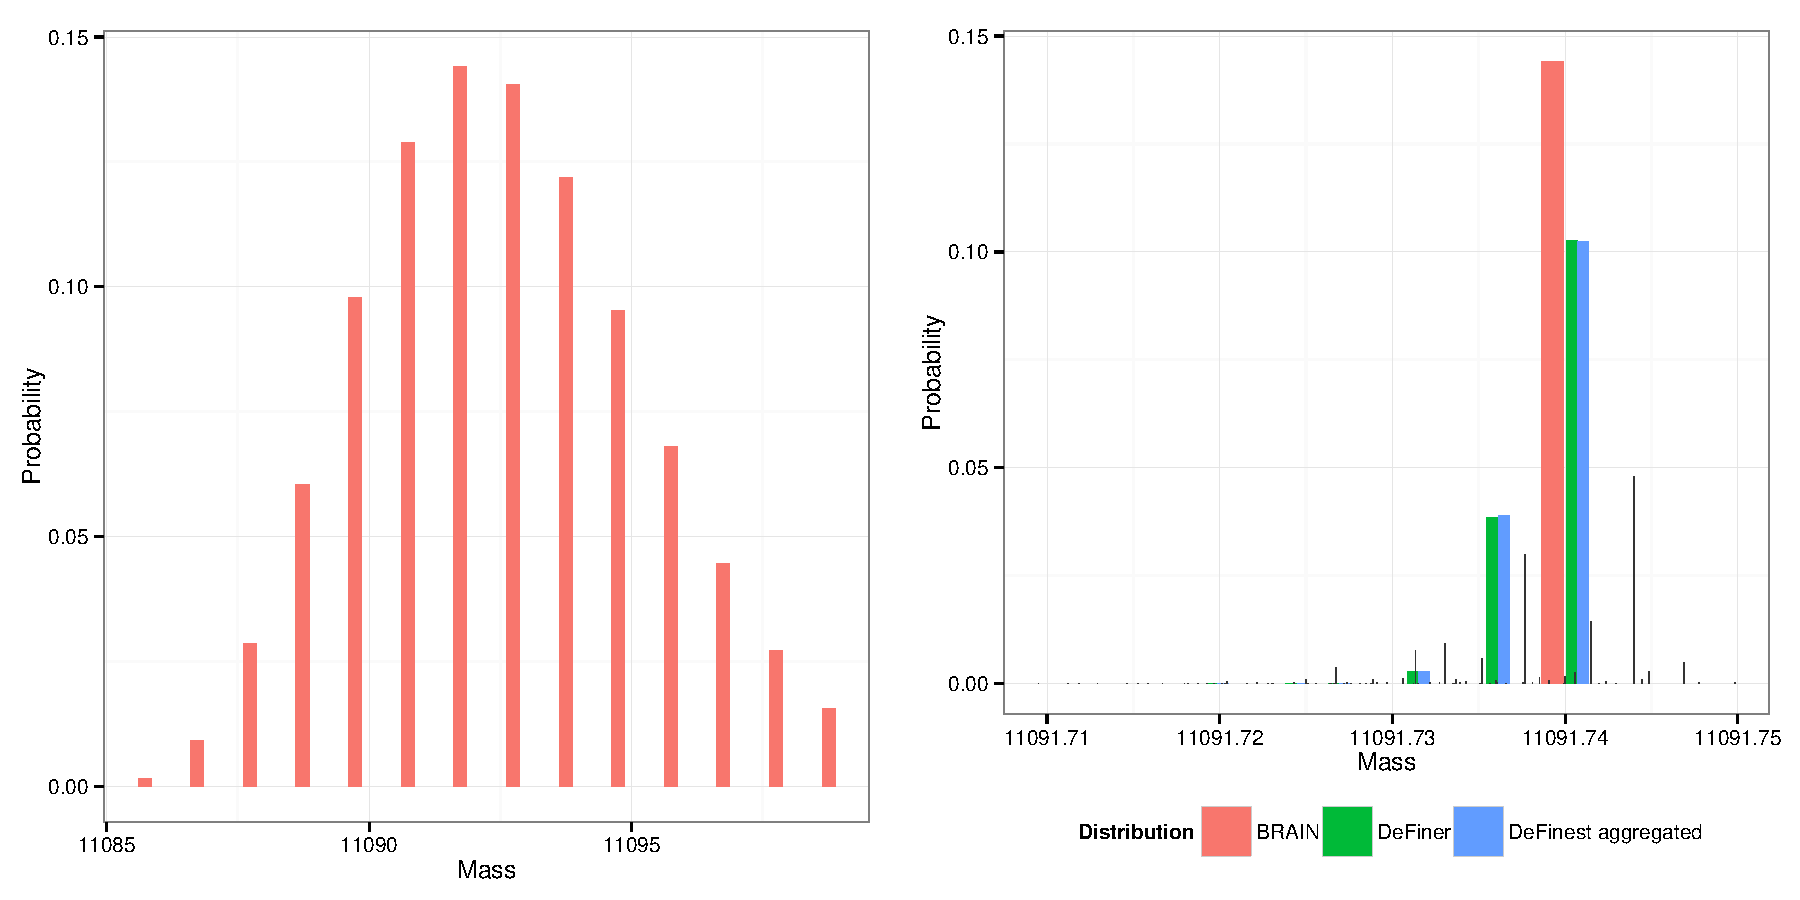
\includegraphics[width=\textwidth]{./img/hierarchyHorizontal}
 \caption{ Peaks in the left pane are probabilities of different $LFS_K$ groups, $K = 0,\dots,13$. In the right pane masses of configurations in $LFS_6$ are plotted: it zooms the region around the tallest peak in the left pane, which is also ploted there for reference. By appropriately aggregating \textsc{DeFiner}'s results, i.e. small black peaks, we calculate the {\it equatransneutronic} precise, non-approximated probabilities. We compare them with \textsc{DeFine}'s results obtained {\it via} the Poisson approximation. There are no apparent differences between them. }
 \label{figure: hierarchy}
\end{figure}


	The potential applications of our results are numerous. For example, having detected a critical set of configurations $A$, s.t. $\MK(A) \approx 95\%$, one might envisage the problem of finding an optimal binning procedure to match real data from a mass spectrometer. In this way, one could measure the machine's resolution without any need to refer to somewhat underdefined notions of {\it p percent valley} and {\it peak width}, see \cite{Eidhammer2008ComputationalMethodsInMassSpectrometry}. 


	Moreover, at least in case of {\it Time of Flight} analyzers, there is an additional advantage of studying the {\it localised fine structure}: it is known, that in these instruments the resolution depends on the mass of analyte, see \cite{Eidhammer2008ComputationalMethodsInMassSpectrometry}. It is more difficult to differentiate correctly between molecules with similar masses, when both of them are big. 


	% However, we judge that all such algorithms could share the idea of using, in one way or another, the approach developed in {\sc Define}: namely, start by choosing a configuration presumed to be in vicinity of the mode of $\MK$, and proceed by a controled {\it breadth first search} until either a certain number of configurations is reached, or they already gathered ones already have enough of probability upon them.

	% A different problem to those mentioned before could be solved in this way to, namely:  

	% \begin{Problem}\label{Big Problem}
	% 	Find a small set $C$ among all possible configurations, s.t. $\mathbb{M}(C) \approx 1$.
	% \end{Problem}

	% The candidate for the biggest peak would by then be the product of modes of each multinomial model in \eqref{product of multinomials}.

	% This problem has been more efficiently be solved by different approaches, e.g. by the use of Fourier transform methods, see \todo{Find Rockwood's publication.}. 



	% Models solving Problem \ref{Big Problem} would have to add some sort of binning procedure with bin width being a function of mass, that not being straightforward to model. Thanks to the localisation in the mass to charge domain, while studying $LFS_K$ we simply neglect that sort of problem.


	Finally, modelling probabilistically the fine structure of the isotopic envelope could serve in an automatic peptide identification procedure. Differences in the fine structure with $K^*$ s.t. $\mathbb{M}_{K^*}(LSF_{K^*}) = \max_K \MK(LSF_K)$ could be particularly informative. However, the design of an appropriate scheme is way beyond the scope of this article.


%!TEX root = ../DeGaulle.tex
\subsubsection*{Acknowledgments.}

We would like to thank Alan Rockwood, Dirk Valkenborg, and, above all -- Piotr Dittwald, for fruitful discussions on the isotopic fine structure related issues.
  \bibliographystyle{./bst/splncs03.bst}
  \bibliography{./bib/spectrometry,./bib/probability,./bib/topology,./bib/generalMath}

  % no \newpage when using \include
%!TEX root = ../DeGaulle.tex
\section*{Tables}

\begin{table}[ht]
	\centering
	\caption{Basic Information on Stable Isotopes, as found in \cite{Rosman1997IsotopicCompositions}.}\label{basic info on isotopes table}
	\begin{tabular}{lccll}
		\toprule
Element 	& Isotope 		& Extra Neutrons& Mass [Da] & Probability 	\\
		\midrule
\multirow{2}{*}{Carbon}  	
			& \ce{^{12}C} 	& 0 			& 12 		& 0.9893 		\\	
  			& \ce{^{13}C} 	& 1 			& 13.0033 	& 0.0107 		\\	
  		\cmidrule(r){1-5}
\multirow{2}{*}{Hydrogen}  	
			& \ce{^1H} 		& 0 			& 1.0078 	& 0.999885 		\\	
  			& \ce{^2H} 		& 1 			& 2.0141 	& 0.000115 		\\	
  		\cmidrule(r){1-5}	
\multirow{2}{*}{Nitrogen}  	
			& \ce{^{14}N} 	& 0 			& 14.0031 	& 0.99632 		\\	
  			& \ce{^{15}N}	& 1 			& 15.0001 	& 0.00368 		\\	  	  
  		\cmidrule(r){1-5}	
\multirow{3}{*}{Oxygen}  	
			& \ce{^{16}O} 	& 0 			& 15.9949 	& 0.99757 		\\	
  			& \ce{^{17}O}	& 1 			& 16.9991 	& 0.00038 		\\	  	  	
  			& \ce{^{18}O}	& 2 			& 17.9992 	& 0.00205 		\\	  	  
  		\cmidrule(r){1-5}	
\multirow{4}{*}{Sulfur}  	
			& \ce{^{32}S} 	& 0 			& 31.9721 	& 0.9493 		\\	
  			& \ce{^{33}S}	& 1 			& 32.9714 	& 0.0076 		\\	  	  
  			& \ce{^{34}S}	& 2 			& 33.9679 	& 0.0429 		\\
  			& \ce{^{36}S}	& 4 			& 35.9671 	& 0.0002 		\\		
		\bottomrule
	\end{tabular}
\end{table}

%!TEX root = ../DeGaulle.tex
\section*{Appendix}

\subsection*{Proof of Lemma \ref{conditional convergence lemma}}

We want to prove that if $\mu^{[n]} \rightharpoonup \mu$ and $\mu^{[n]}(A), \mu(A) > 0$, then also $\mu^{[n]}_A \rightharpoonup \mu_A$. We do this under the assumption that both $\mu^{[n]}$ and $\mu$ are discrete measures on probability space $E$. 

By the {\it Portmanteau Lemma}, see \cite{Kallenberg2002FoundationsOfModernProbability}, $\mu^{[n]} \rightharpoonup \mu$ implies that for any set $A$ with boundry $\partial A$ subject to $\mu( \partial A) = 0$, one should observe 

\begin{equation}\label{convergence in probability on good sets}
	\lim_{n \to \infty} \mu^{[n]}(A) = \mu(A).
\end{equation}


The notion of boundry requires the notion of topology: thus, we decide on the discrete topology, which is natural in this context \footnote{For appropriate topological notions consult \cite{Dugundji1966Topology}.}. In this topology however, $\partial A = \emptyset$, for it is a set theoretical difference of the closure and the interior, both of which are equal to $A$. Hence, $\mu( \partial A) = 0$. Thus, \eqref{convergence in probability on good sets} always holds.

{\it Ex definitione}, $\mu^{[n]} \rightharpoonup \mu$ means, that for any bounded function $f:E\to\mathbb{R}$ one observes
\begin{equation}\label{weak convergence definition}
	\int f \mathrm{d} \mu^{[n]} \underset{n \to \infty}{\xrightarrow{\hspace*{1cm}}} \int f \mathrm{d}\mu\,.
\end{equation}

A simple calculation using both \eqref{convergence in probability on good sets} and \eqref{weak convergence definition} completes the proof:

\begin{equation*}
	\int f \mathrm{d} \mu^{[n]}_A =  \frac{ \int f \mathrm{d} \mu^{[n]} }{ \mu^{[n]}(A) } \underset{n \to \infty}{\xrightarrow{\hspace*{1cm}}} \frac{ \int f \mathrm{d} \mu }{ \mu(A) } = \int f \mathrm{d} \mu\,.
\end{equation*}


\end{document}
